% Graphic for TeX using PGF
% Title: /home/satenske/Diagram1.dia
% Creator: Dia v0.97.1
% CreationDate: Tue Oct 18 17:28:39 2011
% For: satenske
% \usepackage{tikz}
% The following commands are not supported in PSTricks at present
% We define them conditionally, so when they are implemented,
% this pgf file will use them.
\ifx\du\undefined
  \newlength{\du}
\fi
\setlength{\du}{15\unitlength}
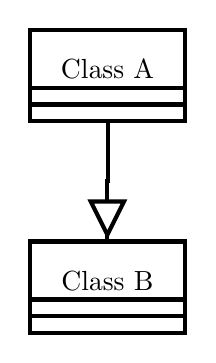
\begin{tikzpicture}
\pgftransformxscale{1.000000}
\pgftransformyscale{-1.000000}
\definecolor{dialinecolor}{rgb}{0.000000, 0.000000, 0.000000}
\pgfsetstrokecolor{dialinecolor}
\definecolor{dialinecolor}{rgb}{1.000000, 1.000000, 1.000000}
\pgfsetfillcolor{dialinecolor}
\pgfsetlinewidth{0.100000\du}
\pgfsetdash{}{0pt}
\definecolor{dialinecolor}{rgb}{1.000000, 1.000000, 1.000000}
\pgfsetfillcolor{dialinecolor}
\fill (6.150000\du,4.150000\du)--(6.150000\du,5.550000\du)--(9.890000\du,5.550000\du)--(9.890000\du,4.150000\du)--cycle;
\definecolor{dialinecolor}{rgb}{0.000000, 0.000000, 0.000000}
\pgfsetstrokecolor{dialinecolor}
\draw (6.150000\du,4.150000\du)--(6.150000\du,5.550000\du)--(9.890000\du,5.550000\du)--(9.890000\du,4.150000\du)--cycle;
% setfont left to latex
\definecolor{dialinecolor}{rgb}{0.000000, 0.000000, 0.000000}
\pgfsetstrokecolor{dialinecolor}
\node at (8.020000\du,5.100000\du){Class B};
\definecolor{dialinecolor}{rgb}{1.000000, 1.000000, 1.000000}
\pgfsetfillcolor{dialinecolor}
\fill (6.150000\du,5.550000\du)--(6.150000\du,5.950000\du)--(9.890000\du,5.950000\du)--(9.890000\du,5.550000\du)--cycle;
\definecolor{dialinecolor}{rgb}{0.000000, 0.000000, 0.000000}
\pgfsetstrokecolor{dialinecolor}
\draw (6.150000\du,5.550000\du)--(6.150000\du,5.950000\du)--(9.890000\du,5.950000\du)--(9.890000\du,5.550000\du)--cycle;
\definecolor{dialinecolor}{rgb}{1.000000, 1.000000, 1.000000}
\pgfsetfillcolor{dialinecolor}
\fill (6.150000\du,5.950000\du)--(6.150000\du,6.350000\du)--(9.890000\du,6.350000\du)--(9.890000\du,5.950000\du)--cycle;
\definecolor{dialinecolor}{rgb}{0.000000, 0.000000, 0.000000}
\pgfsetstrokecolor{dialinecolor}
\draw (6.150000\du,5.950000\du)--(6.150000\du,6.350000\du)--(9.890000\du,6.350000\du)--(9.890000\du,5.950000\du)--cycle;
\pgfsetlinewidth{0.100000\du}
\pgfsetdash{}{0pt}
\definecolor{dialinecolor}{rgb}{1.000000, 1.000000, 1.000000}
\pgfsetfillcolor{dialinecolor}
\fill (6.150000\du,-0.950000\du)--(6.150000\du,0.450000\du)--(9.900000\du,0.450000\du)--(9.900000\du,-0.950000\du)--cycle;
\definecolor{dialinecolor}{rgb}{0.000000, 0.000000, 0.000000}
\pgfsetstrokecolor{dialinecolor}
\draw (6.150000\du,-0.950000\du)--(6.150000\du,0.450000\du)--(9.900000\du,0.450000\du)--(9.900000\du,-0.950000\du)--cycle;
% setfont left to latex
\definecolor{dialinecolor}{rgb}{0.000000, 0.000000, 0.000000}
\pgfsetstrokecolor{dialinecolor}
\node at (8.025000\du,-0.000000\du){Class A};
\definecolor{dialinecolor}{rgb}{1.000000, 1.000000, 1.000000}
\pgfsetfillcolor{dialinecolor}
\fill (6.150000\du,0.450000\du)--(6.150000\du,0.850000\du)--(9.900000\du,0.850000\du)--(9.900000\du,0.450000\du)--cycle;
\definecolor{dialinecolor}{rgb}{0.000000, 0.000000, 0.000000}
\pgfsetstrokecolor{dialinecolor}
\draw (6.150000\du,0.450000\du)--(6.150000\du,0.850000\du)--(9.900000\du,0.850000\du)--(9.900000\du,0.450000\du)--cycle;
\definecolor{dialinecolor}{rgb}{1.000000, 1.000000, 1.000000}
\pgfsetfillcolor{dialinecolor}
\fill (6.150000\du,0.850000\du)--(6.150000\du,1.250000\du)--(9.900000\du,1.250000\du)--(9.900000\du,0.850000\du)--cycle;
\definecolor{dialinecolor}{rgb}{0.000000, 0.000000, 0.000000}
\pgfsetstrokecolor{dialinecolor}
\draw (6.150000\du,0.850000\du)--(6.150000\du,1.250000\du)--(9.900000\du,1.250000\du)--(9.900000\du,0.850000\du)--cycle;
\pgfsetlinewidth{0.100000\du}
\pgfsetdash{}{0pt}
\pgfsetmiterjoin
\pgfsetbuttcap
{
\definecolor{dialinecolor}{rgb}{0.000000, 0.000000, 0.000000}
\pgfsetfillcolor{dialinecolor}
% was here!!!
\definecolor{dialinecolor}{rgb}{0.000000, 0.000000, 0.000000}
\pgfsetstrokecolor{dialinecolor}
\draw (8.020000\du,4.099719\du)--(8.020000\du,2.700000\du)--(8.025000\du,2.700000\du)--(8.025000\du,1.300281\du);
}
\definecolor{dialinecolor}{rgb}{0.000000, 0.000000, 0.000000}
\pgfsetstrokecolor{dialinecolor}
\draw (8.020000\du,3.187916\du)--(8.020000\du,2.700000\du)--(8.025000\du,2.700000\du)--(8.025000\du,1.300281\du);
\pgfsetmiterjoin
\definecolor{dialinecolor}{rgb}{1.000000, 1.000000, 1.000000}
\pgfsetfillcolor{dialinecolor}
\fill (7.620000\du,3.187916\du)--(8.020000\du,3.987916\du)--(8.420000\du,3.187916\du)--cycle;
\pgfsetlinewidth{0.100000\du}
\pgfsetdash{}{0pt}
\pgfsetmiterjoin
\definecolor{dialinecolor}{rgb}{0.000000, 0.000000, 0.000000}
\pgfsetstrokecolor{dialinecolor}
\draw (7.620000\du,3.187916\du)--(8.020000\du,3.987916\du)--(8.420000\du,3.187916\du)--cycle;
% setfont left to latex
\end{tikzpicture}
